% TikZ-based 2XKO Button Notation Diagrams
% Compile separately then include as PDF in main guide
\documentclass[12pt]{article}
\usepackage{tikz}
\usepackage{xcolor}
\usepackage{geometry}
\geometry{margin=1cm}

% 2XKO Colors
\definecolor{viPink}{HTML}{FF69B4}
\definecolor{viPurple}{HTML}{9370DB}
\definecolor{viDark}{HTML}{1A0B1A}
\definecolor{buttonL}{HTML}{FF6B6B}
\definecolor{buttonM}{HTML}{FFE66D}
\definecolor{buttonH}{HTML}{4ECDC4}
\definecolor{buttonS}{HTML}{95E1D3}

\begin{document}

% Page 1: Button Layout Diagram
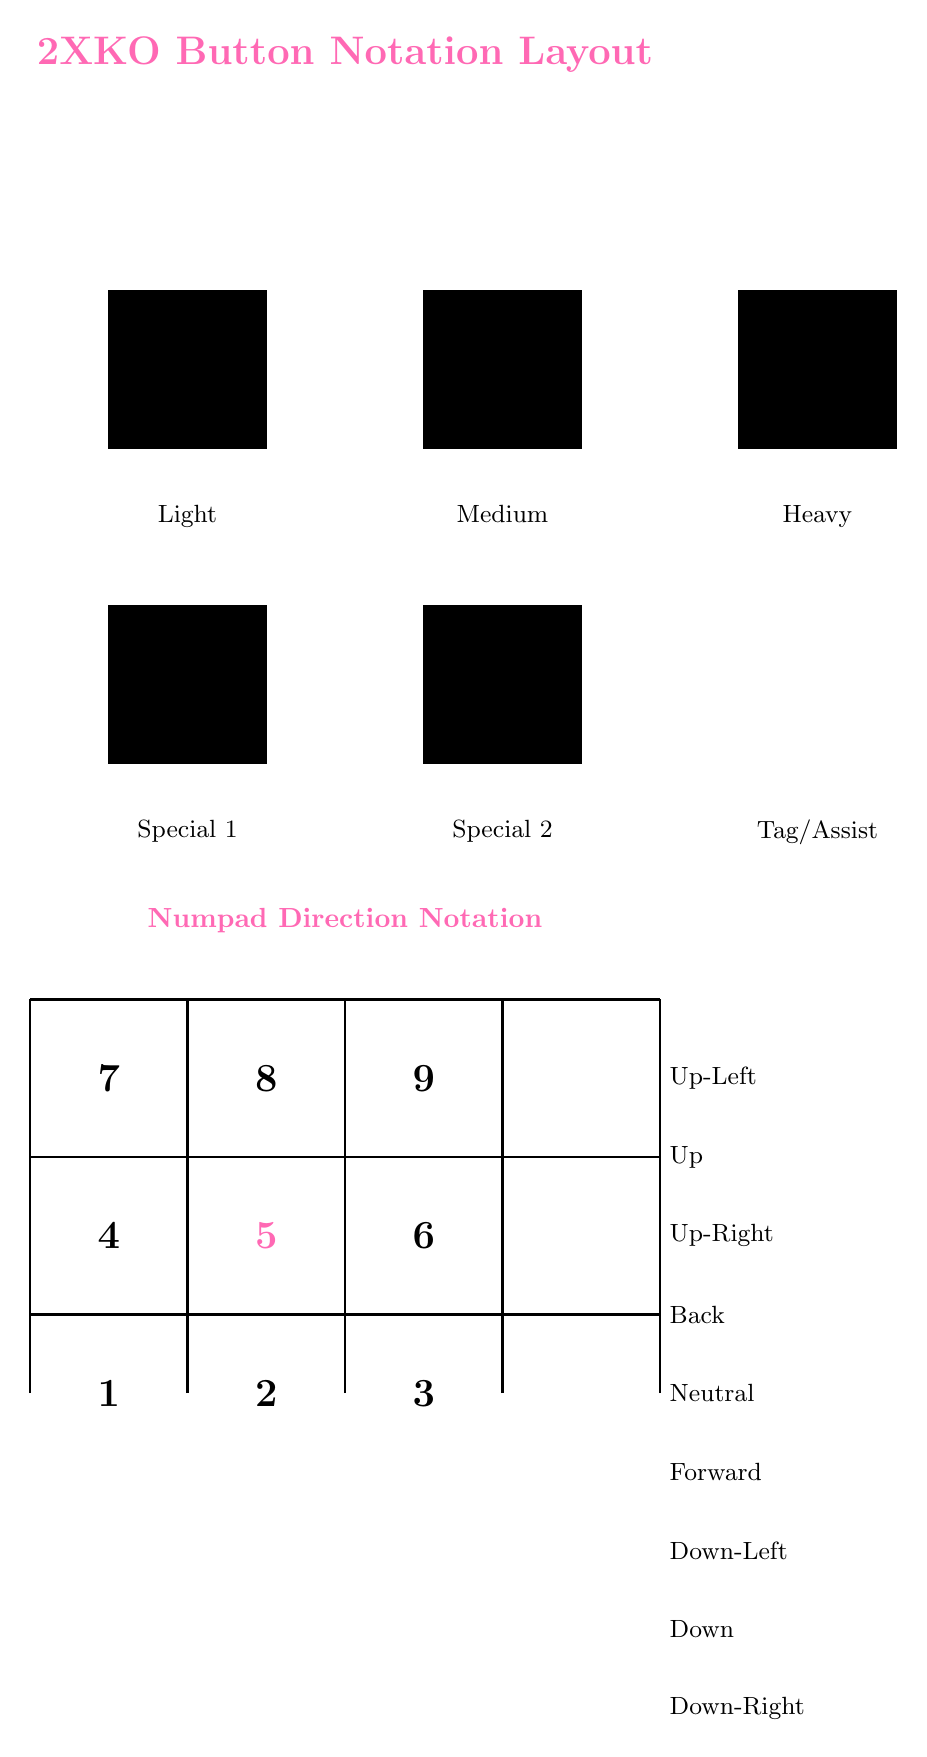
\begin{tikzpicture}[scale=2]
  % Title
  \node[font=\Large\bfseries, color=viPink] at (2, 9) {2XKO Button Notation Layout};
  
  % Controller buttons
  \draw[thick, fill=buttonL, color=black] (0.5, 6.5) rectangle (1.5, 7.5) node[pos=.5, font=\Large\bfseries] {L};
  \draw[thick, fill=buttonM, color=black] (2.5, 6.5) rectangle (3.5, 7.5) node[pos=.5, font=\Large\bfseries] {M};
  \draw[thick, fill=buttonH, color=black] (4.5, 6.5) rectangle (5.5, 7.5) node[pos=.5, font=\Large\bfseries] {H};
  
  \node[anchor=north, font=\small] at (1, 6.2) {Light};
  \node[anchor=north, font=\small] at (3, 6.2) {Medium};
  \node[anchor=north, font=\small] at (5, 6.2) {Heavy};
  
  % Special buttons
  \draw[thick, fill=buttonS, color=black] (0.5, 4.5) rectangle (1.5, 5.5) node[pos=.5, font=\Large\bfseries] {S1};
  \draw[thick, fill=buttonS, color=black] (2.5, 4.5) rectangle (3.5, 5.5) node[pos=.5, font=\Large\bfseries] {S2};
  \draw[thick, fill=viPurple, color=white, line width=2pt] (4.5, 4.5) rectangle (5.5, 5.5) node[pos=.5, font=\Large\bfseries, color=white] {T};
  
  \node[anchor=north, font=\small] at (1, 4.2) {Special 1};
  \node[anchor=north, font=\small] at (3, 4.2) {Special 2};
  \node[anchor=north, font=\small] at (5, 4.2) {Tag/Assist};
  
  % Numpad Notation Guide
  \node[font=\bfseries, color=viPink] at (2, 3.5) {Numpad Direction Notation};
  \draw[thick] (0, 0.5) grid (4, 3);
  
  \node[font=\Large\bfseries] at (0.5, 2.5) {7};
  \node[font=\Large\bfseries] at (1.5, 2.5) {8};
  \node[font=\Large\bfseries] at (2.5, 2.5) {9};
  
  \node[font=\Large\bfseries] at (0.5, 1.5) {4};
  \node[font=\Large\bfseries, color=viPink] at (1.5, 1.5) {5};
  \node[font=\Large\bfseries] at (2.5, 1.5) {6};
  
  \node[font=\Large\bfseries] at (0.5, 0.5) {1};
  \node[font=\Large\bfseries] at (1.5, 0.5) {2};
  \node[font=\Large\bfseries] at (2.5, 0.5) {3};
  
  \node[anchor=west, font=\small] at (4, 2.5) {Up-Left};
  \node[anchor=west, font=\small] at (4, 2) {Up};
  \node[anchor=west, font=\small] at (4, 1.5) {Up-Right};
  \node[anchor=west, font=\small] at (4, 1) {Back};
  \node[anchor=west, font=\small] at (4, 0.5) {Neutral};
  \node[anchor=west, font=\small] at (4, 0) {Forward};
  \node[anchor=west, font=\small] at (4, -0.5) {Down-Left};
  \node[anchor=west, font=\small] at (4, -1) {Down};
  \node[anchor=west, font=\small] at (4, -1.5) {Down-Right};
\end{tikzpicture}

\newpage

% Page 2: Common Notation Symbols
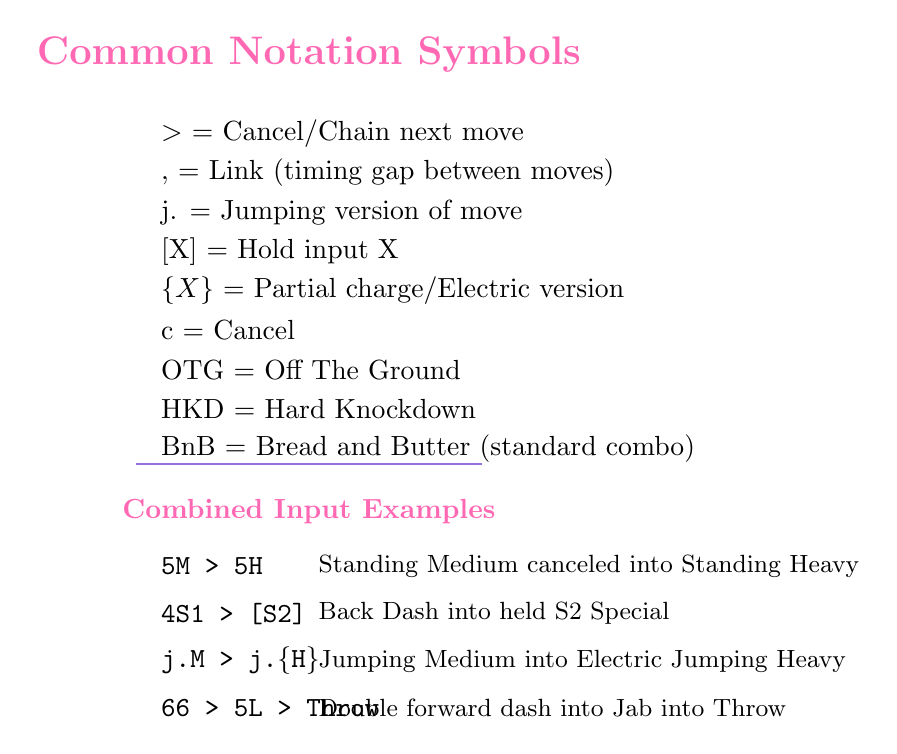
\begin{tikzpicture}
  \node[font=\Large\bfseries, color=viPink] at (2.5, 9) {Common Notation Symbols};
  
  \node[anchor=west, font=\normalsize] at (0.5, 8) {$>$ = Cancel/Chain next move};
  \node[anchor=west, font=\normalsize] at (0.5, 7.5) {$,$ = Link (timing gap between moves)};
  \node[anchor=west, font=\normalsize] at (0.5, 7) {j. = Jumping version of move};
  \node[anchor=west, font=\normalsize] at (0.5, 6.5) {[X] = Hold input X};
  \node[anchor=west, font=\normalsize] at (0.5, 6) {$\{X\}$ = Partial charge/Electric version};
  \node[anchor=west, font=\normalsize] at (0.5, 5.5) {c = Cancel};
  \node[anchor=west, font=\normalsize] at (0.5, 5) {OTG = Off The Ground};
  \node[anchor=west, font=\normalsize] at (0.5, 4.5) {HKD = Hard Knockdown};
  \node[anchor=west, font=\normalsize] at (0.5, 4) {BnB = Bread and Butter (standard combo)};
  
  \draw[color=viPurple, line width=1pt] (0.3, 3.8) -- (4.7, 3.8);
  
  \node[font=\bfseries, color=viPink] at (2.5, 3.2) {Combined Input Examples};
  
  \node[anchor=west, font=\Small\ttfamily] at (0.5, 2.5) {5M > 5H};
  \node[anchor=west, font=\small] at (2.5, 2.5) {Standing Medium canceled into Standing Heavy};
  
  \node[anchor=west, font=\Small\ttfamily] at (0.5, 1.9) {4S1 > [S2]};
  \node[anchor=west, font=\small] at (2.5, 1.9) {Back Dash into held S2 Special};
  
  \node[anchor=west, font=\Small\ttfamily] at (0.5, 1.3) {j.M > j.\{H\}};
  \node[anchor=west, font=\small] at (2.5, 1.3) {Jumping Medium into Electric Jumping Heavy};
  
  \node[anchor=west, font=\Small\ttfamily] at (0.5, 0.7) {66 > 5L > Throw};
  \node[anchor=west, font=\small] at (2.5, 0.7) {Double forward dash into Jab into Throw};
\end{tikzpicture}

\end{document}
